\subsection{Data Generation}
\label{sec:soft_cut_data_generation}

After having trained a recurrent neural net with the existing data, we noticed that the net did not generalize very well.
In order to solve this problem, more data was necessary.
We decided to generate more data by blending random sequences into each other.
A random sequence is picked by reading the gold standard, picking two consecutive elements which encode two cuts with a start and end frame each.
Between the end frame of the first cut and the start frame of the first cut, we can randomly select a subsequence with the desired transition length (11 and 21).
In order to blend two random sequences, we have multiple options for tweening behaviour.
The standard tweening function is linear, but there are also EaseIn, EaseOut etc. (see Figure~\ref{fig:data_generation}).
The tweening function is randomly selected, as well.

In order to achieve further variance in the generated data, we flip the two sequences randomly at the x- or y-axis or at both axes.
With this approach we generated 50 GB of data.


\begin{figure}
    \centering
    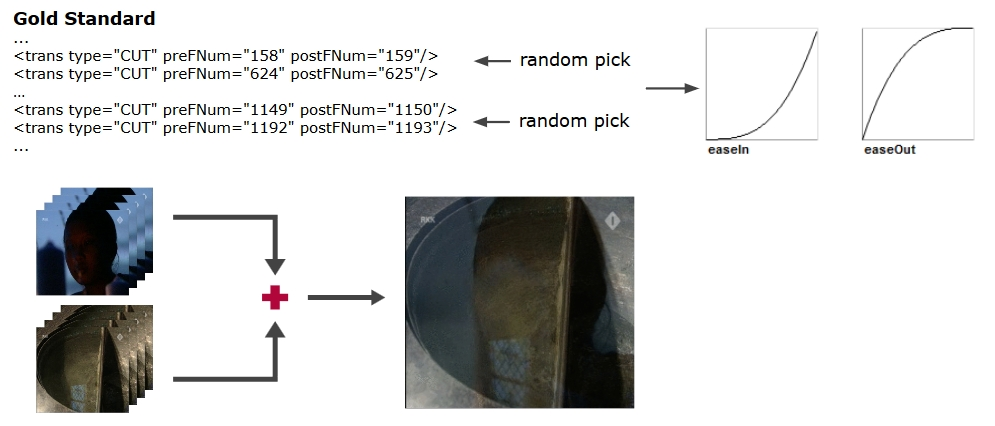
\includegraphics[scale=.5]{images/data_generation.jpg}
    \caption{}
    \label{fig:data_generation}
\end{figure}